% Interaction diagram, LaTeX user level and TeX system software level
% Author: Agostino De Marco
% Based on diagram from Marco Miani and Pascal Seppecher.
\documentclass{article}
\usepackage{tikz}
\usepackage{amsmath,amssymb,amsfonts,amstext}
\usepackage{floatflt}
\usetikzlibrary[arrows,snakes,backgrounds,shapes]
\usetikzlibrary{through}
\usetikzlibrary{calc}
\usepackage{caption}
\usepackage{subcaption}
\usepackage{wrapfig}
\usepackage{makeidx}
\usepackage{transparent}

%%%<
\usepackage{verbatim}
\usepackage[active,tightpage]{preview}
\PreviewEnvironment{tikzpicture}
\setlength\PreviewBorder{5pt}%
%%%>
\usetikzlibrary{positioning}

\newcommand{\ypos}{3}
\newcommand{\xpos}{-.7}
\newcommand{\zpos}{0}

\newcommand{\yslant}{-.3}
\newcommand{\xslant}{.20}

\newcommand{\xoffset}[1]{\xpos*#1+3}
\newcommand{\yoffset}[1]{\ypos*#1}
\newcommand{\zoffset}[1]{\zpos+#1}

\begin{document}
\begin{tikzpicture}[scale=1,every node/.style={minimum size=1cm},on grid]

		\tikzstyle{line} = [draw, thick, -latex',];
		\tikzstyle{commentline} = [draw, dashed, green!50,-latex',shorten >=1pt];
		\draw[gray, dotted] (-1,-2) grid (7,14);
		
	% Software level
%	\begin{scope}[
%		yshift=-120,
%		every node/.append style={yslant=\yslant,xslant=\xslant},
%		yslant=\yslant,xslant=\xslant
%	] 
%		% The lower frame:
%		\draw[black, dashed, thick] (-1.3,0) rectangle (8.2,4.8); 
%		% Agents:
%		\draw[fill=red]  
%			(7.5,2) circle (.1) % .pdf file
%			(5,2) circle (.1) % .ps file
%			(2,2) circle (.1) % .dvi file
%			(-0.5,2) circle (.1); % .tex file
%		% Flows:
%		\draw[-latex,ultra thick,shorten <=5pt,shorten >=5pt] 
%			(-0.5,2) to[out=0,in=-180] (2,2); % latex
%		\draw[-latex,ultra thick,shorten <=5pt,shorten >=5pt] 
%			(2,2) to[out=0,in=-180] (5,2); % dvi2ps
%		\draw[latex-latex,ultra thick,shorten <=5pt,shorten >=5pt] 
%			(5,2) to[out=0,in=-180] (7.5,2); % ps2pdf, pdf2ps
%		\draw[-latex,ultra thick,shorten <=5pt,shorten >=5pt] 
%			(-0.5,2) to[out=90,in=-180] (3.5,3.8) to[out=0,in=90] (7.5,2); % pdflatex
%		\draw[-latex,ultra thick,shorten <=5pt,shorten >=5pt] 
%			(2,2) to[out=90,in=-180] (2.7,3.0) to[out=0,in=-180] (6.7,3.0) to[out=0,in=135] (7.5,2); % ps2pdfm
%		 % Labels:
%		\fill[black]
%			(1.0,2) node[above=-3pt, scale=0.9] {\textsf{\bfseries latex}}			
%			(3.5,2) node[above=-5pt, scale=0.9] {\textsf{\bfseries dvi2ps}}
%			(6.25,2) node[above=-5pt, scale=0.9] {\textsf{\bfseries ps2pdf}}
%			(6.25,2) node[xshift=-1ex,below=-5pt, scale=0.9] {\textsf{\bfseries pdf2ps}}
%			(3.5,3.8) node[xshift=2ex,below=-5pt, scale=0.9] {\textsf{\bfseries pdflatex}}
%			(4.3,3.0) node[xshift=2ex,below=-5pt, scale=0.9] {\textsf{\bfseries dvi2pdfm}}
%			(0.7,0.1) node[above=-2pt, scale=1.1] {\textbf{Software/File level}}
%			(-0.5,2) node[below,scale=.9]{\textsf{\bfseries .tex} file}
%			(2,2) node[below,scale=.9]{\textsf{\bfseries .dvi} file}
%			(5,2) node[below,scale=.9]{\textsf{\bfseries .ps} file}
%			(7.5,2) node[below,scale=.9]{\textsf{\bfseries .pdf} file};	
%	\end{scope}
%	
%	% vertical lines for linking agents on the 2 levels
%	\draw[thick](6.3,5.1) to (6.3,0.9);
%	\draw[thick](3.8,4) to (3.8,-0.32);
%	\draw[thick](0.8,2.4) to (.8,-1.8);
%	\draw[thick](-1.70,1.02) to (-1.70,-3);
%	
	
	
	\begin{scope}[
		yshift=0,
		every node/.append style={yslant=\yslant,xslant=\xslant},
		yslant=\yslant,xslant=\xslant
	]			
			\node[anchor=south,inner sep=0,xshift=0pt,yshift=0pt] at (\xoffset{0},\yoffset{0})
			{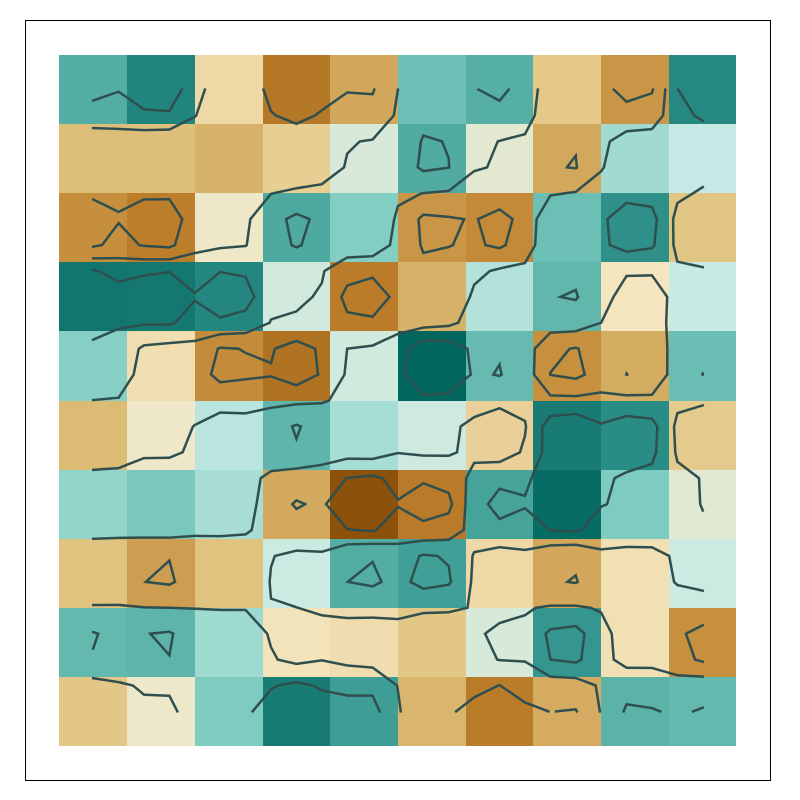
\includegraphics[width=5cm]{c4_.png}};
				
	\end{scope} 
		
	\begin{scope}[
		yshift=0,
		every node/.append style={yslant=\yslant,xslant=\xslant},
		yslant=\yslant,xslant=\xslant
	]
			\node[anchor=south,inner sep=0,xshift=0pt,yshift=0pt] at (\xoffset{1},\yoffset{1})
				{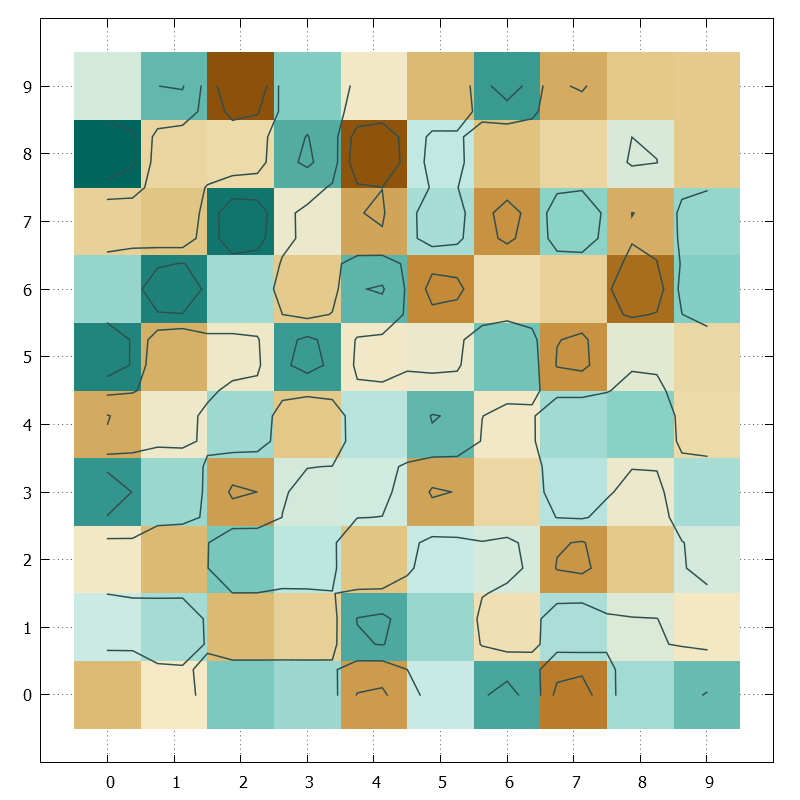
\includegraphics[width=5cm]{c3_.png}};
				
	\end{scope} 
		
	\begin{scope}[
		yshift=0,
		every node/.append style={yslant=\yslant,xslant=\xslant},
		yslant=\yslant,xslant=\xslant
	]
			\node[anchor=south,inner sep=0,xshift=0pt,yshift=0pt] at (\xoffset{2},\yoffset{2})
				{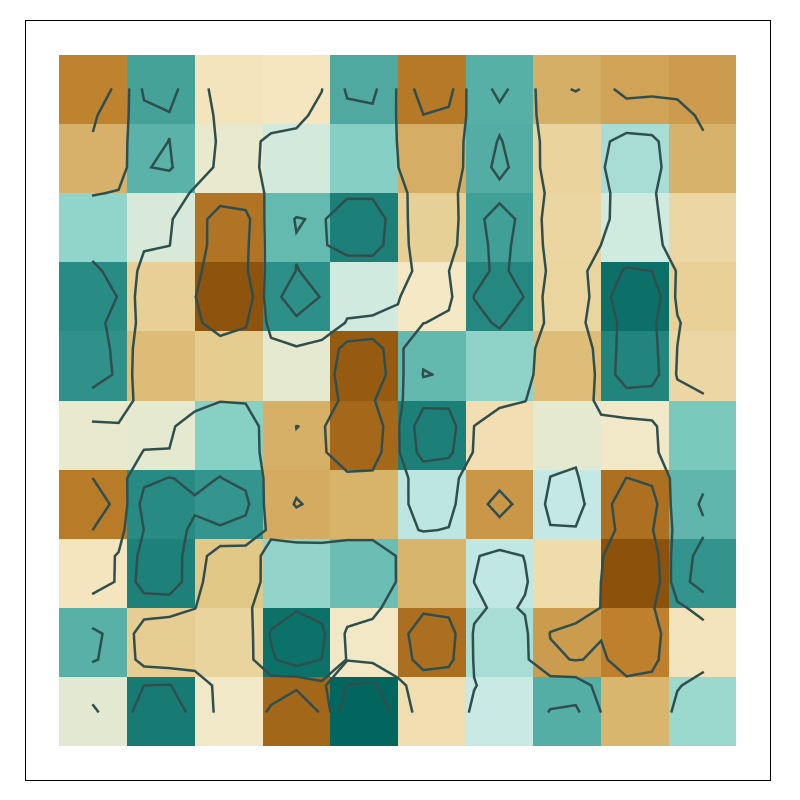
\includegraphics[width=5cm]{c2_.png}};
			
	\end{scope} 
	
	% User level
	\begin{scope}[
		yshift=0,
		every node/.append style={yslant=\yslant,xslant=\xslant},
		yslant=\yslant,xslant=\xslant
	]
			\node[anchor=south,inner sep=0,xshift=0pt,yshift=0pt,fill=white] at (\xoffset{3},\yoffset{3})
				{ 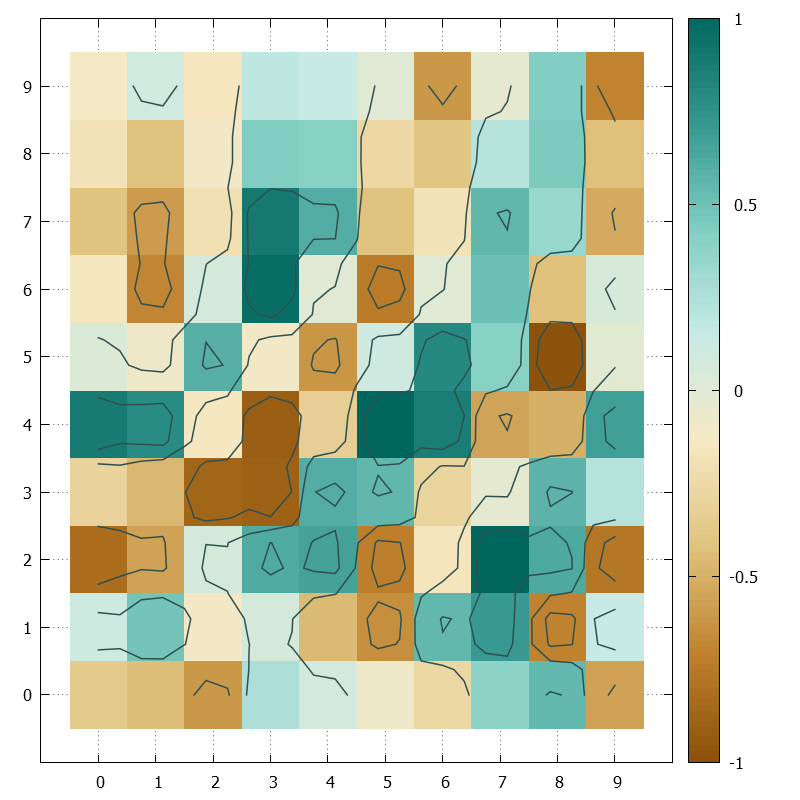
\includegraphics[width=5cm]{c1.png}};
	\end{scope} 


	\begin{scope}[
	%		every node/.append style={yslant=\yslant,xslant=\xslant},
		]
			\node [] (xyz_0) at (0,0){ };
			\node [] (x) at (1,0){ };
			\node [] (y) at (1,1){ };
			\node [] (z) at (0,1){ };
			\node [] (A1) at (0,\zoffset{2.5}){ Antenne 4 };
			\node [] (A2) at (0,\zoffset{5.5}){ Antenne 3 };
			\node [] (A3) at (0,\zoffset{8.5}){ Antenne 3 };
			\node [] (A4) at (0,\zoffset{11.5}){ Antenne 1 };
			\node [] (z_1) at (0,11){};
			
%			\tikzstyle{every path}=[line]
%			\path (xyz_0) -> (x);
%			\path (xyz_0) -> (y);
%			\path (xyz_0) -> (z);
			
	\end{scope} 
		%		% The upper frame:
		%		\fill[white,fill opacity=.70] (-3.1,0) rectangle (9.9,6); % Opacity
		%		\draw[black, dashed, thick] (-3.1,0) rectangle (9.9,6); 
		%		 % Agents:
		%		\draw [fill=red]
		%			(7.5,2) circle (.1) % .pdf file
		%			(5,2) circle (.1) % .ps
		%			(2,2) circle (.1) % .dvi
		%			(-0.5,2) circle (.1); % .tex file
		%
				% the icons
		%				\node[anchor=south,inner sep=0,xshift=-20pt,yshift=10pt,fill=white] at (0,0)
		%					{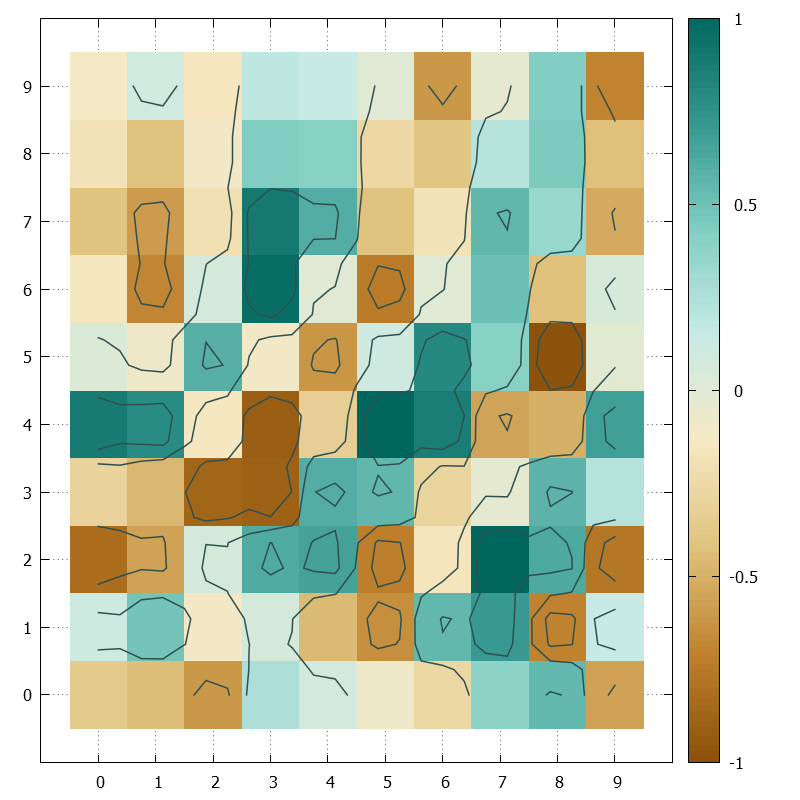
\includegraphics[width=5cm]{c1.png}};
		%					
		%				\node[anchor=south,inner sep=0,xshift=0pt,yshift=8pt] at (2,0)
		%					{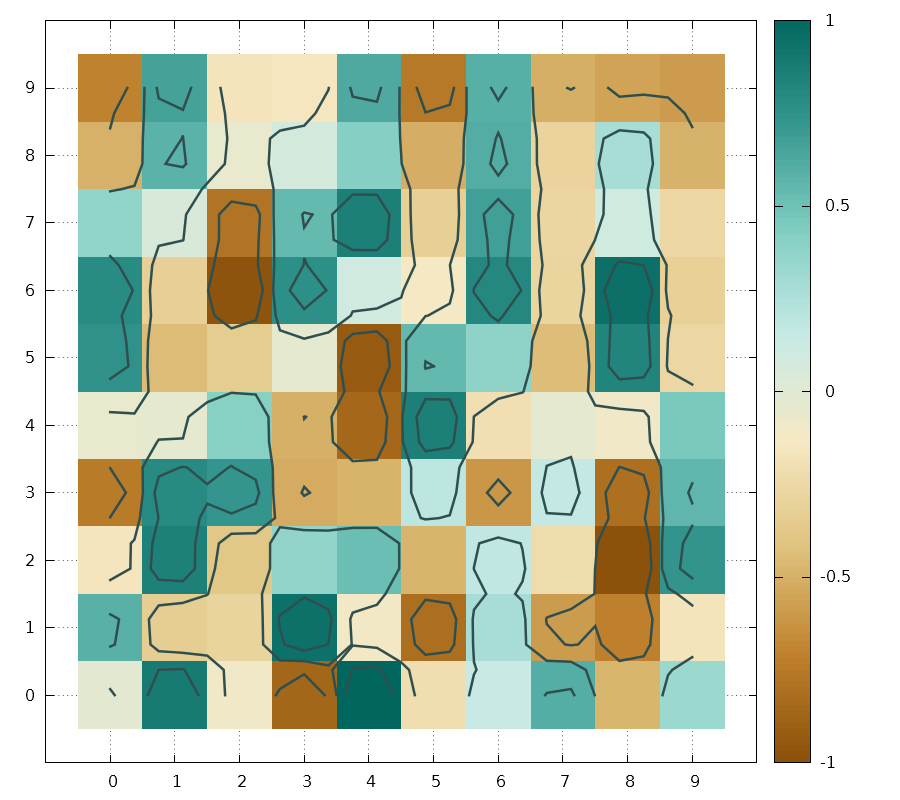
\includegraphics[width=5cm]{c2.png}};
		%					
		%				\node[anchor=south,inner sep=0,xshift=-5pt,yshift=8pt] at (4,0)
		%					{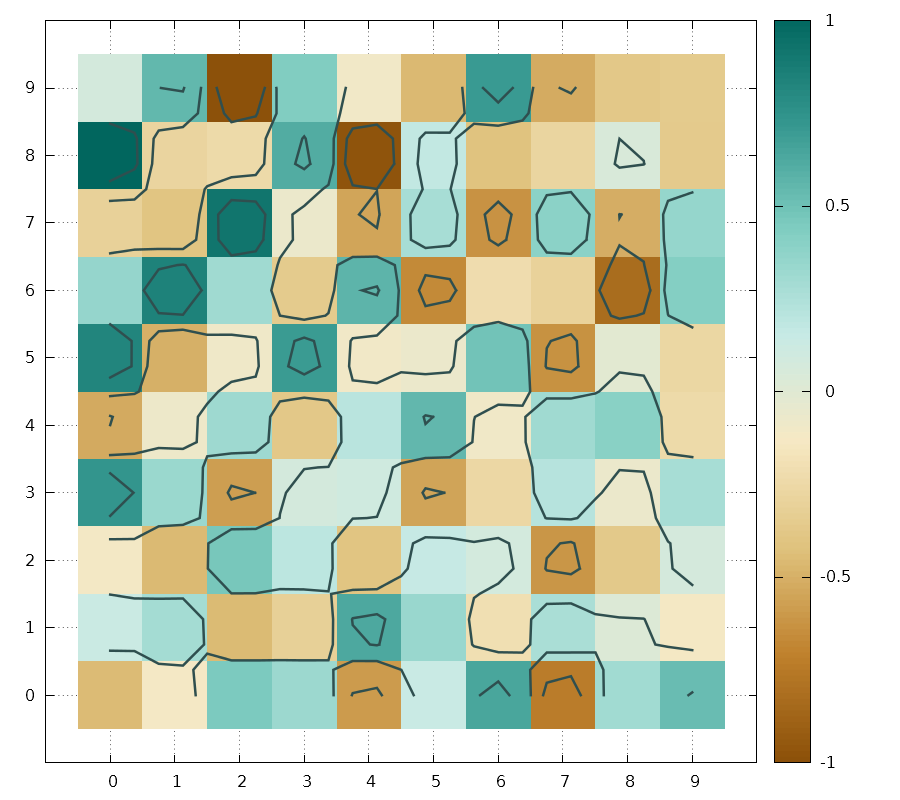
\includegraphics[width=5cm]{c3.png}};
		%					
		%				\node[anchor=south,inner sep=0,xshift=20pt,yshift=8pt] at (6,0)
		%					{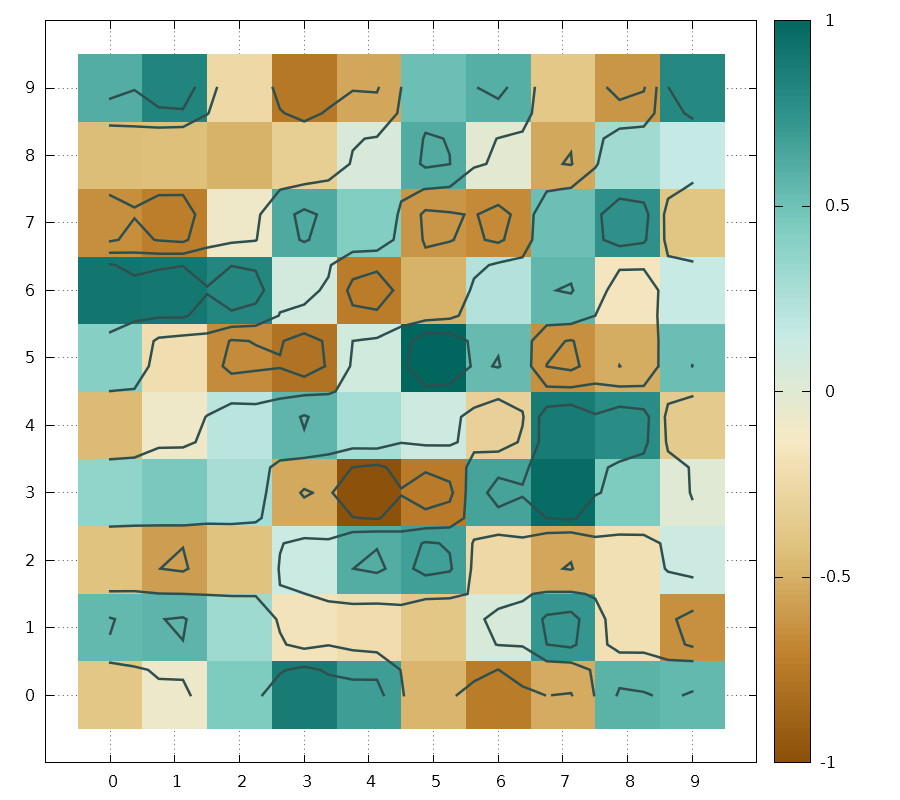
\includegraphics[width=5cm]{c4.png}};
		
					
				
		
		%		\fill[black]
		%			(7.5,2) node[below right,,xshift=-20pt,yshift=-5pt,scale=.9,text width=2.5cm,align=left,fill=white]
		%				{\textsf{\bfseries \mbox{Acrobat Reader}}\\ \textsf{\bfseries SumatraPDF}
		%				\\ \textsf{\bfseries Xpdf}}
		%			(-2.5,5.5) node[anchor=west,inner sep=0, scale=1.1] {\textbf{User level}}
		%			(5.1,1.9) node[below right,xshift=-20pt,scale=.9,text width=2cm,align=left,fill=white]
		%				{\textsf{\bfseries Ghostview}\\ \textsf{\bfseries PSview}\\ \textsf{\bfseries Okular}}
		%			(1.9,1.9) node[below right,xshift=-10pt,scale=.9,text width=2cm,align=left,fill=white]
		%				{\textsf{\bfseries Yap}\\ \textsf{\bfseries Xdvi}}
		%			(-0.5,2) node[below right,xshift=-20pt,yshift=-5pt,scale=.9,text width=2.5cm,align=left,fill=white]
		%				{\textsf{\bfseries \TeX{works}}\\ \textsf{\bfseries \TeX{maker}}\\
		%					\textsf{\bfseries \mbox{\TeX{nic Center}}}} 
		%%		;
\end{tikzpicture}
\end{document}